\documentclass[xcolor=dvipsnames]{beamer}

% ==== 主題 ====
\usetheme{metropolis}
\usefonttheme{professionalfonts}          % 不覆蓋你自訂的字型

% ==== 字型 ====
\usepackage{fontspec}
\usepackage{xeCJK}
\renewcommand{\familydefault}{\rmdefault} % 使用 serif 字體（重點）
\usefonttheme{professionalfonts}

% 西文字型：Times New Roman 的開源替代品
\setmainfont{TeX Gyre Termes}[
  Ligatures=TeX,
  BoldFont={* Bold},
  ItalicFont={* Italic}
]

% 中文字型（可改為思源宋體、標楷體等）
\setCJKmainfont{Noto Serif CJK TC}
\setCJKsansfont{Noto Sans CJK TC} % 有需要再用
\setCJKmonofont{Noto Sans Mono CJK TC}

% ==== 數學字型（與正文字體一致）====
\usepackage{unicode-math}
\setmathfont{TeX Gyre Termes Math}

% ==== 套件 ====
\usepackage{amsmath, amssymb}
\usepackage{graphicx}
\usepackage{hyperref}
\usepackage{minted}
\usepackage{fvextra}
\usepackage{xcolor}
\usepackage{booktabs}

% ==== 顏色設定（可選）====
\definecolor{MyBlue}{RGB}{3, 55, 105}
\setbeamercolor{structure}{fg=MyBlue}
\setbeamercolor{block title}{bg=MyBlue,fg=white}
\setbeamercolor{block body}{bg=blue!5}
\setbeamertemplate{section in toc}{%
  \inserttocsectionnumber.~\inserttocsection\par
}

\setminted{
    linenos,                % 行號
    frame=lines,            % 上下框線
    framesep=5pt,           % 程式碼與邊框距離
    numbersep=8pt,          % 行號與程式碼距離
    fontsize=\scriptsize,   % 字體大小
    breaklines,             % 自動換行
    tabsize=4,              % tab 寬度
    rulecolor=\color{black},% 框線顏色
    xleftmargin=1.5em       % 左側縮排
}

\title{Introduction to STL}
\author{Tai, Wei Hsuan}
\date{week 5}

\begin{document}
	\begin{frame}
		\titlepage
	\end{frame}

    \begin{frame}
        \frametitle{\href{https://drive.google.com/drive/folders/1IN7Dv6ozKHldRXJG6mI0DmjhBlwO6KWK?usp=sharing}{課程簡報}}
        \begin{figure}
            \centering
            
\includegraphics[width=0.7\textwidth]{src/qrcode.png}
        \end{figure}
    \end{frame}

    \begin{frame}
        \frametitle{Outline}
        \tableofcontents
    \end{frame}
    \section{Recap Problems}
    \section{Introduction}
    \begin{frame}{What is STL?}
        STL stands for Standard Template Library, which is a powerful set of C++ template classes and functions that provide data structures and algorithms. It provides a collection of tools for handling any type of data.

        The most poworful feature of the STL is that it allows you handle any type of data, e.g., int, double, string, and even another STL container. This makes it a very versatile and powerful tool for C++ programming.
    \end{frame}
    \begin{frame}{Lecture arrangement}
        This is a series of lectures that will introduce you to the STL and how to use it effectively in your C++ programming.

        In these lectures, we'll cover some common STL components, but not ALL OF THEM. The STL is vast, and we will focus on the most commonly used parts that are essential for competitive programming and general C++ development.
    \end{frame}

    \section{Stack}
    \begin{frame}{What is stack?}
        In English, stack means "a pile of things arranged one on top of another(Cambridge Dictionary)". In C++, stack is a container adapter that gives the programmer the functionality of a stack data structure. 
    \end{frame}

    \begin{frame}{How a stack works?}
        Stack is a Last In First Out (LIFO) data structure. The last element added to the stack will be the first one to be removed.
        
        In other words, you can only access the top element of the stack(i.e., the most recently added element). You can push elements onto the stack, remove elements from the stack, and check the top element of the stack.
        \begin{figure}
            \centering
            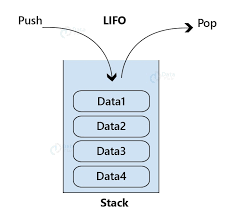
\includegraphics[width=0.5\textwidth]{src/stack.png}
        \end{figure}
    \end{frame}
    
    \begin{frame}[fragile]
        \frametitle{Here are some common operations of stack}
        \begin{minted}{c++}
            stack<int> s; //create a stack of integers
            s.push(1); //push 1 onto the stack
            s.push(2); //push 2 onto the stack
            cout<<s.top(); //print the top element of the stack
            s.pop(); //remove the top element of the stack
        \end{minted}
    \end{frame}

    \begin{frame}[fragile]
        \frametitle{Try these codes}
        \begin{minted}{c++}
            stack<string> s; //create a stack of strings
            s.push("Hello"); //push "Hello" onto the stack
            s.push("World"); //push "World" onto the stack
            cout<<s.top(); //print the top element of the stack
            s.pop(); //remove the top element of the stack
            cout<<s.top(); //print the top element of the stack
        \end{minted}
        What will be the output of the above code? Why? Is it reasonable?
    \end{frame}
    \section{Practice Problems}
    \begin{frame}
        \frametitle{Practice}
        In this section, the following problems are provided:
        \begin{itemize}
            \item i213, a565 are simple problems
            \item c123, c700, j607 are complex problems
            \item r395 is a hard problem
        \end{itemize}
        Choose suitable problems depending on your level.
    \end{frame}
\end{document}